\documentclass{standalone}
\usepackage{tikz}
\begin{document}
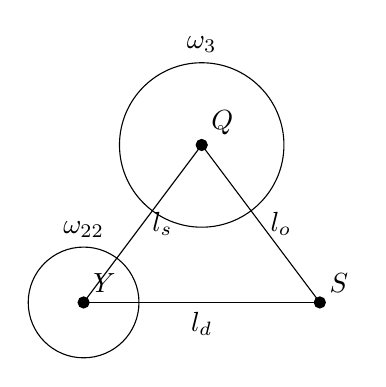
\begin{tikzpicture}[scale=1.0]
  \filldraw (0.0, 0.0) circle (2pt) node[above right] {$Y$};
  \filldraw (3.0, 0.0) circle (2pt) node[above right] {$S$};
  \filldraw (1.5, 2.0) circle (2pt) node[above right] {$Q$};
  \draw (0.0, 0.0) -- (3.0, 0.0) node[midway, below] {$l_d$};
  \draw (1.5, 2.0) -- (0.0, 0.0) node[midway, right] {$l_s$};
  \draw (3.0, 0.0) -- (1.5, 2.0) node[midway, right] {$l_o$};
  \draw (1.5, 2.0) circle (1.0443) node[above=1.0443cm] {$\omega_{3}$};
  \draw (0.0, 0.0) circle (0.7032) node[above=0.7032cm] {$\omega_{22}$};
\end{tikzpicture}
\end{document}